\documentclass{article}

\usepackage {amsmath}
\usepackage {textcomp}
\usepackage {setspace}
\usepackage [pdftex]{graphicx}
\usepackage[sort&compress]{achemso}
%\usepackage{lineno}

\usepackage[
top    = 0.5in,
bottom = 1.0in]{geometry}
%left   = 2.50cm,
%right  = 2.50cm]{geometry}

% some formatting tags
%\oddsidemargin  0.0in
%\evensidemargin 0.0in
%\textwidth      6.5in

\title{Dancing on Water: The Choreography of Sulfur Dioxide Adsorption to Aqueous Surfaces}
\author{Eric S. Shamay \and Kevin E. Johnson \and Geraldine L. Richmond}

\begin{document}


\newcommand{\suldiox}{SO$_2$}
\newcommand{\ang}{\,$\textrm{\AA}$}
\newcommand{\angs}{\ang}
\newcommand{\wat}{H$_2$O}
%\newcommand{\deg}{$\,^{\circ}$}

\maketitle

%\onehalfspacing
%\linenumbers 
\doublespacing


\begin{abstract}
One might expect the high surface tension of water to be a barrier to absorption of a gas into the liquid phase, but we know that gaseous adsorption onto, and subsequent absorption into a water surface is a common phenomenon on this planet.  What is not commonly known is how an atmospheric gas such as \suldiox~and molecules at the water surface can overcome the barrier created by strong water-water surface bonding interactions.  What this interplay looks like, the distances from the water surface at which these attractive interactions begin, and how they influence the orientational nature of both \suldiox~and surface water molecules is the focus of this computational study.  The results fill a void in the information about this system existing from previous experimental studies by providing information about the dimensional nature of the gas-surface interactions, and the details of how the two species twist and turn orientationally with increased surface interactions.  Classical molecular dynamics have been employed in both equilibrium and steered molecular dynamics (SMD) simulations for \suldiox~at a neat-water surface, and at a surface with high interfacial \suldiox~concentrations.  The results provide new molecular insights for understanding the interaction of this prevalent gas on aerosols and other aqueous surfaces in the environment.
\end{abstract}

\section{Introduction}

The doorway to the uptake of a gas by an aqueous solution is the water surface. Although we know much about the behavior of a gas on either side of that entrance, far less is known about how that surface acts to attract, facilitate, or thwart the transit of a molecule between the two bulk phases. What is the interplay between the gas and surface water molecules, and when does one begin to influence the behavior of the other? What species form during gas adsorption onto liquid surfaces, and what are the intermediary steps?  Is molecular orientation of either the gas or surface molecules a factor in the adsorption process? Are specific gas or liquid molecular orientations necessary for gaseous adsorption?  Experimental studies to address such questions are valuable but do not provide the full resolution necessary to determine the geometries of adsorbing gases, or to determine the orientations of the molecules at the liquid surface near the adsorption site. This type of information can be determined computationally, and when coupled to the experimental studies can provide a more comprehensive picture of the gas-liquid surface adsorption process.

An important gas for developing a picture of gaseous adsorption and entry into a water surface is sulfur dioxide.\cite{Donaldson1995,Lattanzi2010,Shah2011,Tzivian2011,Johns2011,Faloona2009,Jurkat2010,Wu2011,Jayne1990,Jayne1990a,Yang2002} \suldiox~enters the environment as an important industrial product, and also naturally through terrestrial processes. Atmospheric dust particles and gases have been implicated in the oxidation of \suldiox, and act as reaction surfaces for chemical mechanisms that are still poorly understood.\cite{Baltrusaitis2011,Rubasinghege2010,Li2007,Madsen2008,Boniface2000} \suldiox~acts as a major component of atmospheric pollution, and is a precursor to acid rain formation, and cloud nucleation. Its high solubility in water makes \suldiox~an integral compound in many aqueous atmospheric reactions, as well.  Obtaining a more complete picture of the \suldiox~adsorption process is important for understanding gaseous adsorption of this environmentally important gas on water and aerosol surfaces as well as being a model system for understanding the more general nature of gases at aqueous interfaces.

In this work we provide a molecular picture of \suldiox~adsorption on a water surface.  This study demonstrates the strong orientational effect of surface water molecules on the adsorbing gas during the approach and entry into the surface region at both high and low \suldiox~surface concentrations.  These computational studies complement and significantly expand the picture developed in our recent experimental vibrational sum frequency spectroscopy (VSFS) studies of \suldiox~adsorption of aqueous solutions of various compositions and temperatures,\cite{Tarbuck2005,Tarbuck2006} and the subsequent studies using both classical and ab initio simulations.  These experimental studies showed that an \suldiox~surface hydrate complex forms when an aqueous surface is exposed to \suldiox~gas. The computational study by Baer et al.\cite{Baer2010} then made a series of predictions of the specific nature of the hydrated complex through classical and ab initio simulations. That work developed a detailed picture of the nature of the \suldiox~surface complex with water, and related it to the surface water OH vibrational IR spectra.  The most recent experimental studies have shown that whereas the binding of gaseous \suldiox~to a water surface is greatly enhanced at cold temperatures, the reversibility of the adsorption process remains.\cite{Ota2011}  Complementary experiments showed that low pH aqueous environments inhibit the bulk reactions of \suldiox, but do not affect the surface binding or its reversibility.  What is apparent in the VSF spectra obtained in all of these experiments is the tendency of water to reorient upon surface bonding, with the effect becoming more pronounced at high \suldiox~surface concentrations. Since the \suldiox~molecule was not specifically probed, conclusions on how \suldiox~bonding contributes to reorienting surface water molecules and the orientation of \suldiox~itself upon approach and surface bonding could only be inferred. 

To fill this void, the computational studies described herein provide a detailed picture of the orientation of both \suldiox~and surface water molecules during the adsorption process.  The depth profiling studies which examine the orientation of both species during the approach and entry of the gas into the interfacial region are obtained using equilibrium and steered (SMD) classical molecular dynamics simulations. The latter approach involves steering a gas molecule into the aqueous phase, and characterizing its molecular orientation as it transits through the interfacial region.  This unique approach enables new insights into the behaviors of gas molecules as they move near to liquid water. We also simulate how \suldiox~adsorption occurs on a water surface saturated with adsorbed \suldiox, analogous to the conditions of the \suldiox~experimental studies recently performed.\cite{Ota2011} The results of this study provide an intimate perspective on the adsorption of \suldiox~at an aqueous surface, and a more complete picture of gaseous adsorption to liquid interfaces.

\section{Computational Approach}

Molecular dynamics simulations were performed using the Amber 11 software suite.\cite{Case2010} Polarizable models for the \wat~and \suldiox~molecules were used in the simulations, and have been used previously in studies on interfacial systems because they are known to more accurately reproduce interfacial structure and free energy profiles.\cite{Wick2007,Rivera2006,Dang1998} The \wat~model used is the POL3 water model (also discussed in the supplemental information),\cite{Caldwell1995} and for \suldiox~we used the model of Baer et al. that places a single polarizable center on the sulfur atom.\cite{Baer2010} An intermolecular cutoff of 12\angs~was used for long-range electrostatic forces. The simulations were performed in the NVT ensemble using Langevin dynamics for temperature control. Induced dipoles were treated by the polarizable potential functions of the Amber molecular dynamics software.

All simulations began with an equilibrated cube of 900 \wat~molecules, with sides of length 30\angs. The long axis of each simulation cell (the axis normal to the water surface) was then lengthened to 120\angs, and the systems were further equilibrated for 10 ns. The simulations all employed periodic boundaries to create an ``infinite-slab'' geometry. After equilibrating the neat-\wat~slabs two types of systems were created by introducing \suldiox: a single-\suldiox~system, herein referred to as the ``neat-water'' system, and a ``saturated'' \suldiox~system with many gaseous surface and bulk-water \suldiox~molecules.

The low and high concentration simulated systems, ``neat-water'' and ``saturated'', respectively, were created as follows: the neat-water simulation involved the addition of a single \suldiox~molecule either within the bulk of the water slab (for equilibrium MD), or above the slab surface (in the SMD simulations). The single-\suldiox~neat-water system was then evolved for 2 ns to produce an equilibrated starting configuration. Because of the extremely low concentration of \suldiox~in the neat-water system the surface waters behave similarly to a true neat-water air-liquid interface. The neat-water system orientational results shown later in this work reproduce well the results of our previous orientational studies of surface water behavior.\cite{Walker2006b,Hore2008} The saturated system had 22 \suldiox~molecules introduced to the water slab bulk in order to saturate it to a level coinciding with the Henry's law constant for \suldiox~in water (k\textdegree$_H = 1.4$ mol/kg*bar).\cite{Lide2000} Additionally, 50 \suldiox~molecules were introduced into the gas phase outside of the saturated water slab to simulate an added \suldiox~gas pressure. The additional gas in the vapor phase was added over the course of several ns to keep a constant 1 atm of \suldiox~pressure above the water surface as \suldiox~gas molecules adsorbed to the surface. The saturated system with both bulk and gaseous \suldiox~was then evolved for 2 ns to produce a starting configuration for further saturated simulations.

\subsection{Equilibrium Molecular Dynamics Simulations}

Equilibrium simulations involved adding \suldiox~to a water slab and equilibrating as outlined above. The neat-water system had a single \suldiox~added to the center of the water box, representing a concentration of 0.06 M. The more concentrated ``saturated'' system consisted of 22 \suldiox~molecules in the bulk corresponding to a concentration 1.35 M. This saturated system was exposed to an additional 50 \suldiox~in the gas phase above the water surface. After equilibration for 2 ns, both the low and high concentration systems were then evolved for a further 10 ns data collection using a time step of 0.5 fs, with atomic coordinates recorded every 100 fs.

\subsection{Steered Molecular Dynamics Simulations}

% need to add in the specifics about the SMD routine, force constants, calculations, etc.
A second set of simulations began with an equilibrated water slab as in the surface equilibrated method above. However, in both the neat-water and saturated starting systems, a single \suldiox~was introduced 20\angs~above the water slab surface, with the sulfur atom tethered to its initial position. The systems were then evolved for 1 ns, taking coordinate snapshots every 20 ps to create 50 starting points for further simulations. Steered molecular dynamics (SMD) were then performed on the 50 system configurations (in both the neat-water and saturated configurations) to guide the \suldiox~down towards a tethered water near the water slab's center of mass by applying a small steering force to the \suldiox-sulfur atom. This steering technique has been previously developed and used to successfully model chemical events.\cite{Isralewitz2001,Giorgino2011,Bizzarri2011,Strzelecki2009,Patargias2009,Liu2006} The \suldiox~thus passed through the continuum of environments from gas phase to (neat- and saturated) water surface adsorption, and finally absorption into the bulk of the \wat~slab. Each of the SMD simulations were performed for a total of 200 ps, using a time step of 1 fs, and taking snapshots of the system every 25 fs. Figure \ref{fig:starting-configurations} illustrates two sample starting configurations for the SMD simulations, showing both the neat-water slab and the saturated slab configurations before steering the \suldiox~towards the water bulk.

A separate set of SMD simulations were performed with tethering of one of the \suldiox-oxygens to the water slab center of mass. This was done to ensure that the orientation of the \suldiox~during the adsorption transit was not an artifact of the choice of atom used for tethering. The simulations produced the same results (not shown) for the orientational analyses, so the data from the original tethering scheme was used.

\begin{figure}[h!]
	\begin{center}
		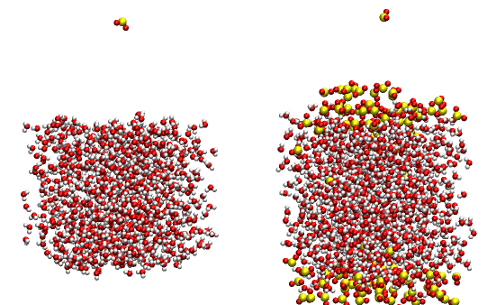
\includegraphics[scale=1.0]{startingconfigurations.png}
		\caption{Sample starting configurations for the two types of SMD simulations. The neat-water slab simulation introduces a single \suldiox~molecule that is then guided into the surface of the water and further into the bulk (left). The saturated slab simulation begins with a water system that has been loaded with \suldiox~to saturate the water phase, and also with a high pressure of \suldiox~gas (right). The single \suldiox~(shown at the top) is then steered through the surface region saturated with \suldiox~molecules, and into the water bulk.}
		\label{fig:starting-configurations}
	\end{center}
\end{figure}

\subsection {Aqueous Surface Location}

	The first portion of the studies involved creating orientational depth-profiles in the interfacial region comprised of \suldiox~and \wat~upon exposure and adsorption of the gas. Recognizing that a liquid surface is a dynamic boundary that is neither flat nor stationary, we must define a reference point in the interfacial region which we refer to here as the water surface location. Several previous studies have used the technique of fitting a line shape to the averaged density profile of the water, and extracting interfacial shape and location parameters to define the water surface location.\cite{Shamay2010,Wick2006c,Chowdhary2006} Hyperbolic tangent functions have been used often, and values for the ``Gibb's dividing surface'' location, and interfacial width have thus been determined.\cite{Matsumoto1988} However, in long simulations the location and shape of the interface changes, and the motion of surface waters alters the interfacial width at any given time step. Thus, the density profile fitting will capture averaged widths and locations, not instantaneous values. Similarly, the averaged values of location and width will obscure information about any drift or deformations the surface undergoes. The analysis presented here attempts to retain these subtleties through the use of a ``corrected'' coordinate system.
	
Figure \ref{fig:density-flaw} demonstrates the problem of surface location drift during a simulation (even with utilizing the Amber NSCM parameter). Figure \ref{fig:density-flaw}A shows the density profile of water and \suldiox~over the course of one of the 10 ns trajectories used in this work using the original uncorrected coordinates of the system taken from the raw atomic positions of the molecular dynamics data output. The water density profile and location (thin gray line in Figure \ref{fig:density-flaw}A) is produced by averaging the instantaneous density profile at each time step in the simulation over all the time steps. The water profile was then fit to a $\tanh$ function (black line) to extract the position and width parameters of the water surface. The fitted surface water density profile has a width of 3.77\angs, which is comparable to values reported for similar neat-water systems.\cite{Dang1997,Hore2008} A bulge in the gas-phase ($\leq 52$\angs) side of the water density profile is indicative of the drift of the water slab over the course of the trajectory. Thus the calculated location and width from the $\tanh$ line fit are not accurate over long trajectories for defining a stationary reference point. 

	To overcome this problem we define the water surface location by calculating a reference location at each time step by averaging the positions of the waters contained in the topmost monolayer. This provides a consistent and intuitive reference point in the simulations to which we relate our analyses, but does not increase the computational burden. The number of waters included in the averaging is determined by taking a few issues into account. First, counting the waters found in the topmost cross-section of the water slab over several time steps indicated between 65-75 waters that established a full monolayer. This was done by a visual inspection of the slab using the VMD MD visualization package.\cite{Humphrey1996} Alternatively, assuming a spherical model of water with a radius of 2.2\angs, two layers of hexagonally tight-packed spheres yielded a similar number of surface water molecules. Increasing the number of waters used in calculating the surface location diminishes the effects of the few waters that briefly rise above the surface into the gas phase, stabilizing both the surface position and thickness values. Taking the close-packed model as a maximum number of waters fit into a flat surface, the topmost 70 water molecules were used for calculating instantaneous water surface locations for each simulation step. 
  
This method for finding the outer monolayer location was implemented, and the surface location is plotted as a function of simulation time in Figure \ref{fig:density-flaw}B. It is apparent from the surface location plot that the water slab location, and thus the surface location, drifts over the 10 ns, spanning approximately 12 \angs. However, the maximum standard deviation of the positions of the waters comprising the surface layer at each time step is only 1.85 \angs. Consequently, all depth locations in our analyses are calculated relative to the instantaneous surface location at the corresponding time step of the trajectories.

\begin{figure}[h!]
	\begin{center}
		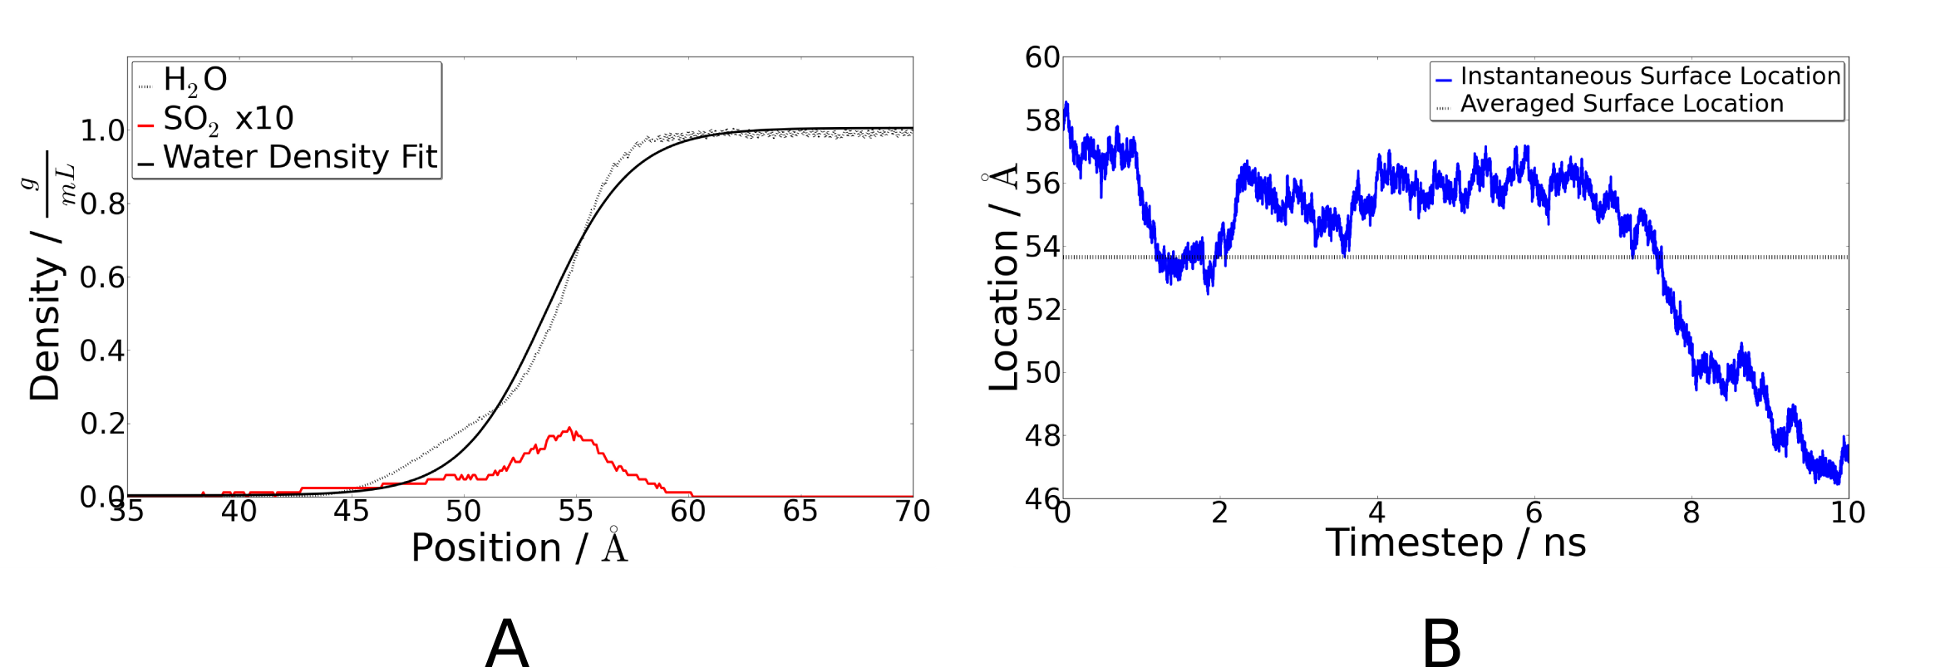
\includegraphics[scale=1.0]{density-location.png}
		\caption{(A) Density profiles of \wat~(Gray) and \suldiox~(red) from a 10 ns simulation of the neat-water system with a single sulfur dioxide. The \wat~density profile was fit using a hyperbolic tangent function (black) to extract location and width data for the water surface. Position values are based on the atomic position data of the water oxygens and \suldiox~sulfurs from the raw molecular dynamics output. (B) The instantaneous location of the outer \wat~monolayer was calculated for each simulation time step (blue), and the surface location extracted from the density fitting was also shown for reference (horizontal dashed line). Long simulations of liquid slabs result in drift of the slab location, and the consequent broadening of the water density profile if the surface location is not determined repeatedly throughout the simulation.}
		\label{fig:density-flaw}
	\end{center}
\end{figure}


  %Taking one of the simulations of the neat-water slabs, a series of calculations were performed to find the averaged positions and the standard deviations of varying numbers of the topmost waters. It was found that using 70 waters produced a standard deviation of the water positions corresponding to a width of 3.2\angs. as reported by Baer et al.when fitting the density profile with a hyperbolic tangent lineshape. To match the interfacial width of Baer using the standard deviation of our simulations, 70 water molecules would have to be included in the top monolayer. Thus, the calculations and analyses presented in this work incorporate 70 water molecules when calculating the surface location.


\subsection{Molecular Orientation}

Knowing the molecular orientation of both the \wat~and \suldiox~is a prerequisite for understanding the chemistry occurring during the \suldiox~adsorption process. With the surface location as defined above, the simulated systems were analyzed to characterize the orientation of \wat~and \suldiox~in various environments above, within, and below the aqueous surface region. The two molecules studied are similarly shaped with a C2$_v$ axis along their bisectors, and a molecular plane defined by three atoms. A body-fixed frame is defined for both \wat~and \suldiox~as shown in Figure \ref{fig:molecular-frame}. In each analysis a space-fixed reference axis is used that corresponds to the long axis of the system's periodic cell normal to the plane of the water surface. The orientational analyses presented herein focus on two angles used to define molecular orientation. The molecular orientation angles $\theta$ and $\phi$ are determined from a set reference axis as shown in Figure \ref{fig:water-angles}A.
	
	The ``tilt'' angle, $\theta$, defines the angle formed between the molecular bisector vector (the molecular z-axis, pointing from the central atom in the direction of the other two atoms) and the positive system reference axis. Thus the value of $\theta$ falls within a range of [0\textdegree,180\textdegree]. An angle of $\theta=$ 0\textdegree~indicates a molecule with its bisector aligned with the reference axis, while $\theta=$ 180\textdegree~results from an anti-aligned configuration. Sample representations of molecular orientations resulting from different values of $\theta$ are shown in Figure \ref{fig:water-angles}B.
	
	A second angle, $\phi$, defines the molecular ``twist'' of the molecule. $\phi$ is the angle of rotation around the molecular bisector axis that quantifies the rotation of the molecular plane with respect to a plane perpendicular to the water surface. The values of $\phi$ fall in the interval [0\textdegree,90\textdegree] because of the symmetry of \wat~and \suldiox~molecules with respect to twist about their bisector axes. For values of $\theta \approx$ 90\textdegree, $\phi$ provides additional information about whether the molecular orientation is ``flat'' to the surface (e.g. the plane of the molecule is aligned with the plane of the surface), or if it is perpendicular. The values of $\phi$ for different molecular orientations are depicted in Figure \ref{fig:water-angles}C. %However, the symmetry of the \wat~and \suldiox~molecules create equivalence between the two H, or O, atoms (in the \wat~or\suldiox, respectively). $\phi=-\pi$ is equivalent to $\phi=\pi$, and both situations are equivalent to $\phi=0$. Because $\phi=-\phi$, the value is reported within the range of $[0,\frac \pi 2]$. 
	Values of $\theta$ close to 0\textdegree~or 180\textdegree~result in an isotropic distribution in $\phi$ because of the symmetry of the plane of the surface in directions perpendicular to the surface normal reference axis.

%	The two molecules studied, \wat~and \suldiox, and similarly shaped with a C2$_v$ axis along their bisectors, and a molecular plane is defined by their three atoms. The orientational analyses presented herein focus on two angles used to define the molecular orientation in space. In each analysis a reference axis is used to define molecular angles, and is the z-axis unless otherwise specified. A ``tilt'' angle, $\theta$, defines the angle formed between a vector (generally the bisector vector pointing from the central atom in the direction of the other two atoms) and the positive reference axis. Thus the value of $\theta$ falls within a range of $[0,\pi]$. A second angle, $\phi$, defines the molecular ``twist'' around the reference axis. $\phi$ is formed between the projection of a vector onto the x-y reference plane, and the x-axis. $\phi$ is thus defined relative to the x-axis, and its values are in the interval $[-\pi,\pi]$. However, because of the symmetry of the \wat~and \suldiox~molecules and the equivalence of the two H or O atoms (in the \wat~or\suldiox, respectively), $\phi=-\pi$ is equivalent to $\phi=\pi$, and both situations are equivalent to $\phi=0$. Because $\phi=-\phi$, the value is reported within the range of $[0,\frac \pi 2]$. Figure \ref{fig:spherical-angle} shows the angle definitions using the z-axis as the reference axis.

\begin{figure}[h!]
	\begin{center}
		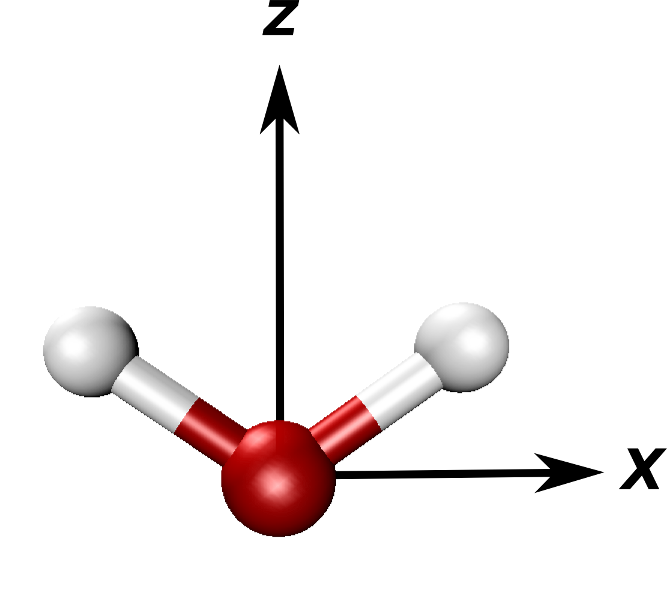
\includegraphics[scale=1.0]{molecularframesmall.png}
		\caption{Molecular body-fixed axes are defined with the x-z plane formed by the three atoms, and the z-axis aligned to the molecular bisector. The y-axis is normal to the molecular plane, and one of the bonds points in the positive x direction.}
		\label{fig:molecular-frame}
	\end{center}
\end{figure}

\begin{figure}[h!]
	\begin{center}
		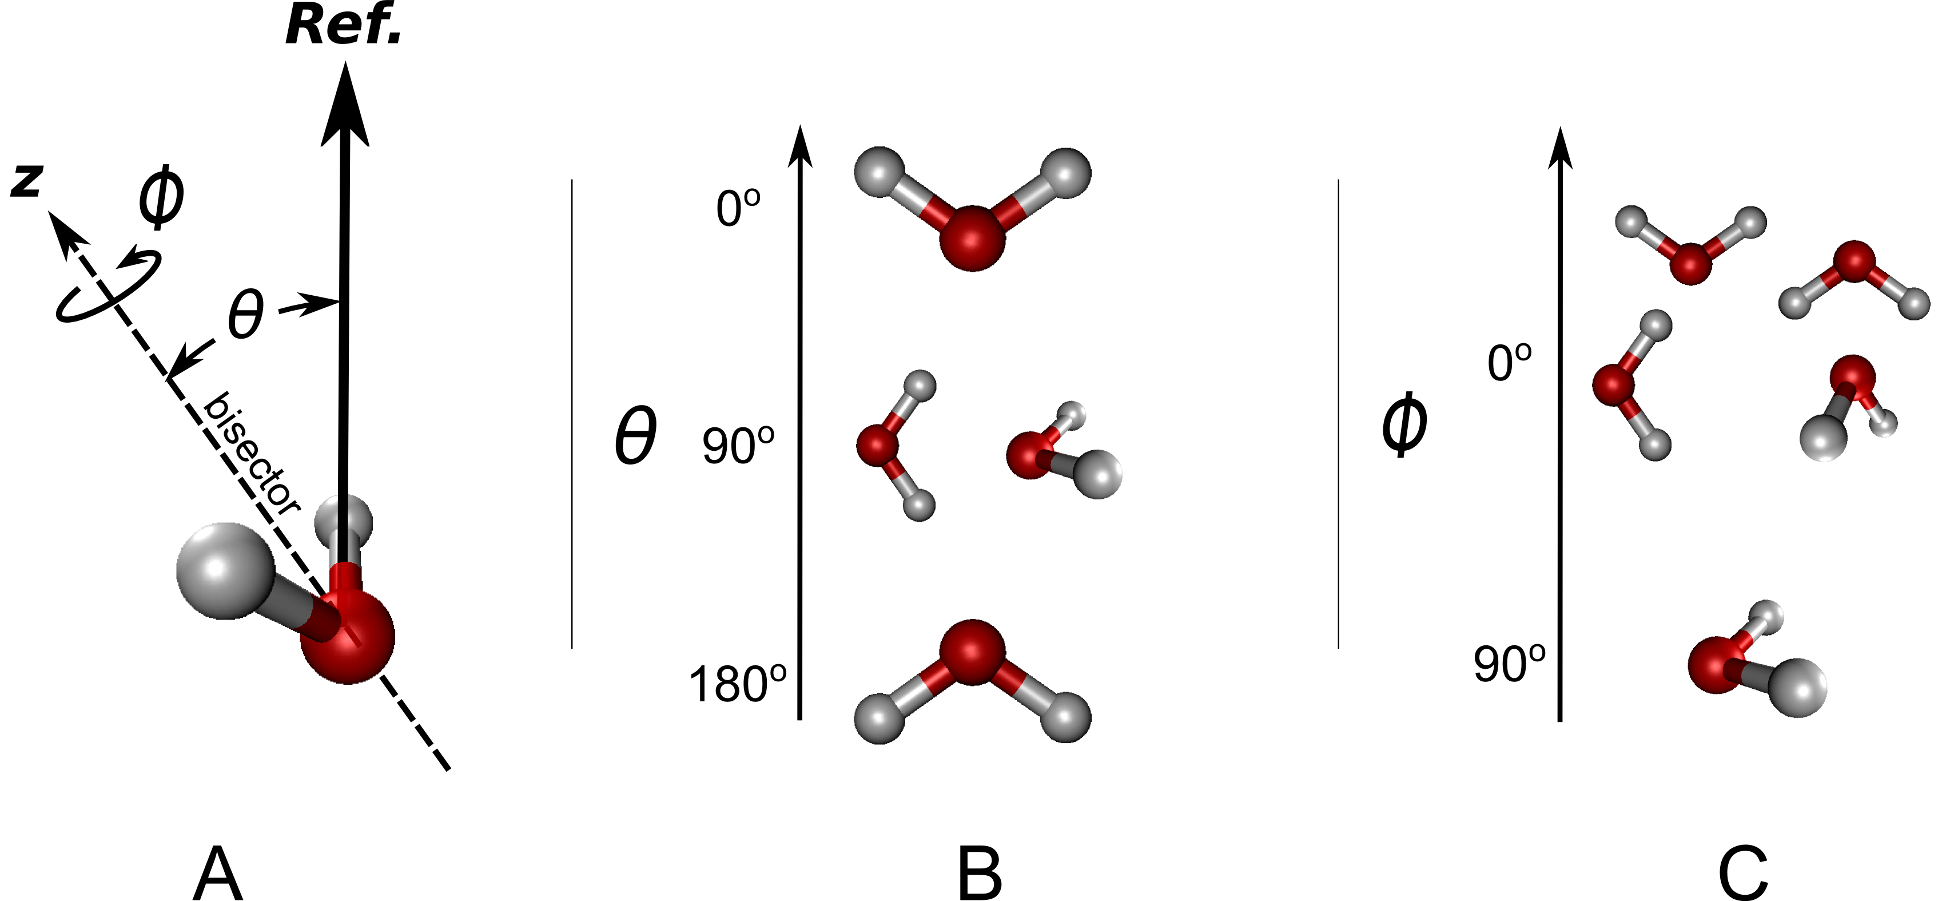
\includegraphics[scale=1.0]{molecular-angles-small.png}
		\caption{(A) The definition of the angles $\theta$ and $\phi$ used to define molecular orientation of \suldiox~and \wat~relative to a reference axis. (B) $\theta$ is the value of the ``tilt'' of the molecular bisector from the reference axis, with $\theta$ values ranging from  0\textdegree~(aligned) to 180\textdegree~(anti-aligned). $\theta = $ 90\textdegree~aligns the bisector parallel to the plane of the water surface. Several bisector orientations are shown depicting different $\theta$ values. (C) $\phi$ is the ``twist'' angle defined as a rotation around the molecular bisector axis. A value of 0\textdegree~aligns the plane of the molecule perpendicular to the plane of the water surface. A value of 90\textdegree~rotates the molecule to lie flat in the plane of the water surface. Because of the symmetries of \suldiox, \wat, and the plane of the water surface, the range of $\phi$ values is limited to 0\textdegree~$\leq \phi \leq$~90\textdegree.}
		\label{fig:water-angles}
	\end{center}
\end{figure}


\subsection{Surface Density Distributions}

One measure of surface activity is the spatial distribution of molecules in the interfacial region. The density distributions of both \wat~and \suldiox~were calculated for the equilibrium MD simulations. The results presented in Figure \ref{fig:density} show both the water (black) and \suldiox~(red) density distributions, averaged over the two simulated interfaces of each slab. As shown, the single \suldiox~in the neat-water system remained at the water slab surface. The \suldiox~in the saturated system accumulated mostly at the surface, but some residual \suldiox~remained well into the bulk water.

%The density distributions of the \suldiox~were fit to gaussian lineshapes as shown in equation \ref{eq:gaussian} using the common definitions of the variables $A$, $\mu$, and $\sigma$, and given as a function of the distance to the top surface, $z$.

%\begin{equation}
%  \rho(z)=\frac{A}{\sqrt{2 \pi \sigma^2}} e^{-\frac{(z-\mu)^2}{2\sigma^2}}
%  \label{eq:gaussian}
%\end{equation}

In the simulated neat-water slab, the \suldiox~molecular density distribution concentrates near the water surface location, indicating an affinity for the interfacial region. During the course of the simulation, the \suldiox~does not venture into the bulk water nor does it escape the water surface into the gas phase, but remains located within 5-\angs~of the surface region. This is consistent with what is found experimentally in our laboratory using VSFS,\cite{Tarbuck2005,Tarbuck2006} and also supported by the computational simulations and spectral calculations of Baer et al.\cite{Baer2010} The experimental studies indicated that upon exposure of \suldiox~to a \wat~surface, a layer of solvated \suldiox~forms, modifying the structure of water in the upper surface region. In the experimental system, the \suldiox~bonding interaction with the free OH oscillators is manifested in a red-shift of the free OH frequency indicative of a bonding interaction. 

The saturated solution simulation results indicate that under the high concentration of \suldiox, the \suldiox~accumulation at the surface is increased. However, unlike the neat-water slab, the saturated slab has a non-zero bulk concentration of \suldiox. The added concentration of \suldiox~creates a layer of molecules bound to the top of the water surface. The center of the \suldiox~density distribution is further into the gas phase than for the neat-water surface with a single-\suldiox~molecule. Additionally, the water profile is broader in the saturated system. This indicates that water penetrates into the \suldiox~layer, and moves further into the gas phase than under the neat-water conditions. Because of the limitations of the classical model in accurately reproducing the first hydration shell around the \suldiox, we do not draw specific conclusions about the hydrated surface complex's geometry. However, the surface affinity of the hydrated \suldiox~is well reproduced by both the classical and ab initio methods.\cite{Baer2010}

\begin{figure}[h!]
	\begin{center}
		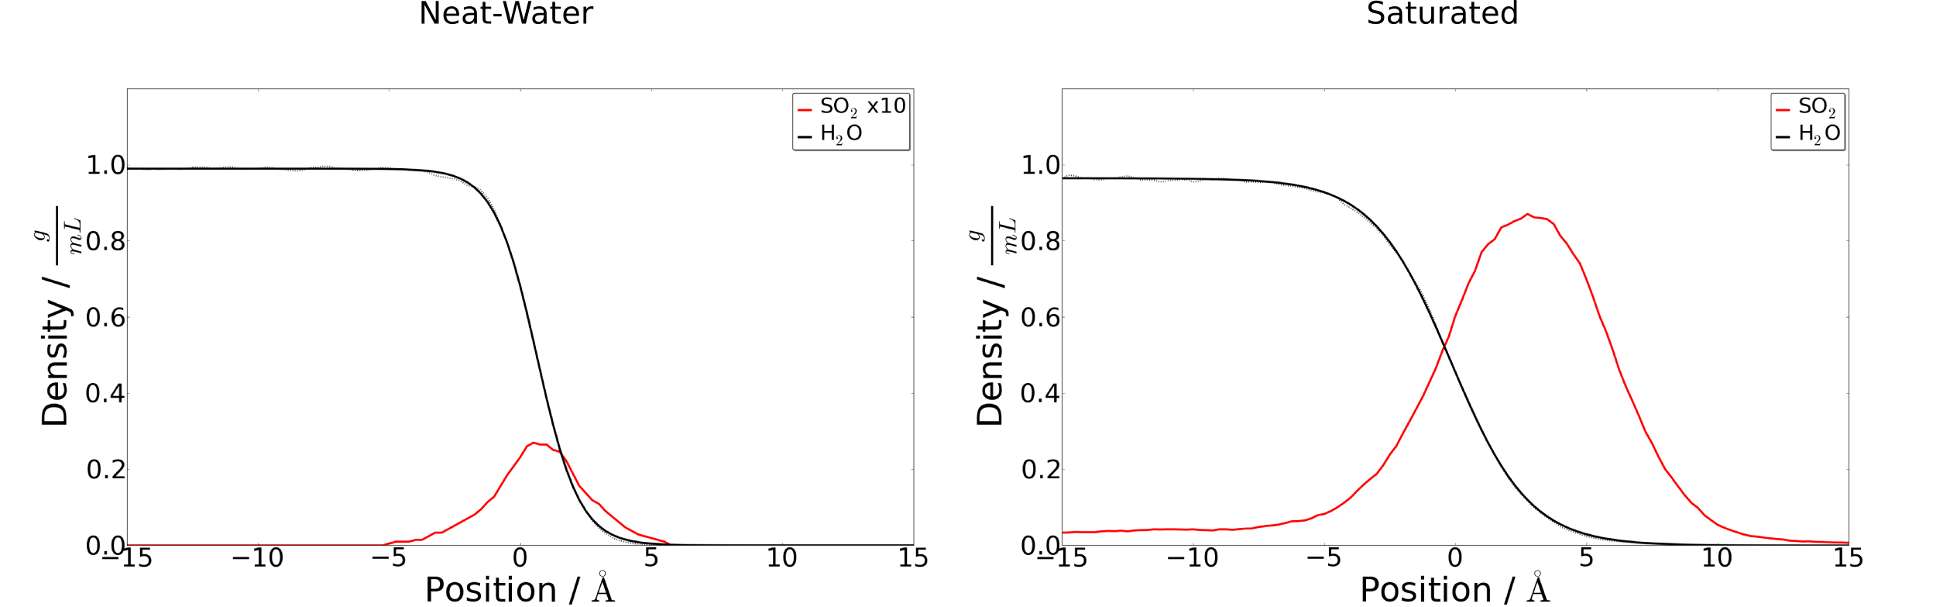
\includegraphics[scale=1.0]{density.png}
		\caption{Molecular density distributions of \wat~(black) and \suldiox~(red) calculated along the long-axis of the simulated cells. The position axis shows the distance from the instantaneous surface location of the \wat~slab, with positive values located above the slab towards the gas phase, and negative values located in the water bulk. Distributions of both the neat-water simulation with a single \suldiox~(left, with the \suldiox~density scaled 10x for clarity), and the saturated system (right) are shown.}
		\label{fig:density}
	\end{center}
\end{figure}

\subsection{Equilibrated MD}

Geometric analyses were performed to characterize the net molecular orientation of \wat~and \suldiox~molecules at different depths from the water surface location. At each distance from the surface location, an orientation profile was created for both the \wat~and \suldiox~molecules. The bi-variate orientation distributions for the angles $\theta$ and $\phi$ at various depths were combined to form the intensity plots that show how the molecular orientation distributions change with distance to the surface location. These plots (Figures \ref{fig:water-orientation}, \ref{fig:so2-orientation}, and \ref{fig:so2-transit-angles}) allow for a visual interpretation of how the net orientations are affected when moving from the gas phase through the interfacial region and to the surface location, and then further into the aqueous interfacial region and bulk. Both the neat-water, with only a single \suldiox~introduced, and the high-concentration saturated system were analyzed. In the case of the neat-water system, the introduction of a single \suldiox~does not greatly affect molecular orientation of water molecules in the interfacial region. These results of the water orientation are very similar to a neat-water system without any adsorbed solutes (not shown).

The depth profile plots are arranged as a grid of 2D histograms. Each histogram is calculated for all molecules falling within a particular depth in the water interfacial region. The depth of each plot is marked (in \ang) in the upper-right, with the water surface location set at 0\angs, positive depths lie on the gas-phase side of the surface, and negative depths are on the bulk water side. The horizontal axes of each histogram represent $\theta$ values, and the vertical axes represent $\phi$ values. Areas of low intensity appear in dark blue, and highest intensity in dark red. Regions of the plots where the intensity (coloration) is equally distributed along either the vertical or horizontal axes are considered isotropic in $\phi$ or $\theta$, respectively. Likewise, areas of the plot with high intensity over a small orientational range are considered to exhibit an orientational preference at the given depth. The angle distributions from both simulated slab surfaces were averaged for all the orientation analyses.

\subsubsection{\wat~Orientation}

The orientation depth-profiles for \wat~are shown in Figure \ref{fig:water-orientation} for both the neat-water (top) and saturated (bottom) systems during the equilibrium MD simulations. The interfacial region for both these calculations and the VSF experiments is defined as the region where molecular orientational anisotropy exists around the surface water location. Fitting the water density profiles we have calculated an interfacial width of approximately 10\angs~for the neat-water system, and approximately 16\angs~for the saturated system. In both systems the strongest orientational preference is found at the slab surfaces (positions near 0\angs). Previous work on orientational preference of water at air surfaces shows the same trend as our neat-water results.\cite{Walker2006b,Hore2008} The swaths of coloration indicating high intensity appearing in the neat-water plots from -4 to +4\angs, (and the corresponding regions in most of the saturated system plots) show the overall preference of water to orient at the surface. The plots of the neat-water and saturated systems are similar to each other with a narrow region of reorientation, but the effect in the interfacial region is greater in the neat-water system as evidenced by the sharper transition in intensity from blue to red, compared to the saturated system that has a less pronounced intensity change over larger areas of the histograms.

The bisector tilt of the water molecules, $\theta$, concentrates around $\theta=$ 90\textdegree within the first few\angs~above and below the water surface location, becoming progressively isotropic further through the interfacial region and into the water bulk of both systems. Above the surface location at positive distances, $\theta \leq$ 90\textdegree~indicates that the water hydrogens tend to point towards the gas-phase side of the surface. As the tilt nears $\theta=$ 90\textdegree~the \wat~bisector lies within the plane of the surface indicating a water orientation either flat on the surface, or with some amount of ``twist'' sending the OH bonds in towards, or out of the bulk. The value of $\phi$ determines the ``twist'' in this case. Both systems show a similar trend where waters at or just below the surface have values of $\phi$ near 90\textdegree, and waters above the surface take on values of $\phi$ near 0\textdegree. This jump in the angular distribution of $\phi$ indicates that waters at or below the surface lie mostly flat in the plane of the interface, and as they move above the surface towards the gas phase, they reorient with one OH bond pointing towards the water bulk, and one pointing out of the surface into the gas. This behavior is more strongly pronounced in the neat-water system where most of the surface waters are not interacting with an adsorbed layer of \suldiox~molecules.

%This result agrees somewhat with a recent air/water study by Fan et al. in which the surface orientations of several water models were analyzed.\cite{Fan2009} They simulated water using non-polarizable models, however, which alters the behavior of water at interfacial regions when compared to the polarizable POL3 model used in our work. The main conclusions are similar in that one OH tends to point further into the air phase than the other, but differs in that this effect is less pronounced with the polarizable model.

Although the plots show overall similarities for both the neat-water and saturated systems, the presence of a layer of adsorbed \suldiox~molecules alters the orientation of those waters furthest into the gas phase. For the saturated solution, the resulting orientation of waters above 0\angs, shown in the bottom set of plots of Figure \ref{fig:water-orientation}, is nearly isotropic in $\phi$, and with $\theta \leq$ 90\textdegree. This results from waters with bisectors pointing further into the adsorbed \suldiox~gas layer, and both hydrogens pointing outward from the aqueous bulk. The effect is more pronounced as the waters move further from the water surface, and above 4\angs~the $\theta$ distribution is mostly concentrated around $\theta=$ 0\textdegree (see Figure \ref{fig:water-angles}).

%The histograms show overall similarities for both systems in their shapes and intensities from approximately 0\angs~and below. The presence of a saturated layer of adsorbed \suldiox~molecules, however, alters the water orientation, but not necessarily the orientational depth of the interface. In both $\theta$ distributions, the orientations of waters in the bulk region are isotropic until 5\angs~below the surface location. At 5\angs~below the surface the water molecules begin to orient with their bisectors within the plane of the interface (perpendicular to the surface normal, $\cos(\theta)\approx 0$). The corresponding location in the plot of $\phi$ shows that those molecules are also mostly flat to the surface ($\cos(\phi)\approx 1$). Moving further out from the bulk and into the gas phase, the distributions show $\cos(\theta)$ increasing. Waters further out from the bulk have fewer bonding interactions, and orient with their hydrogens more towards the gas phase. The bisector pointing further into the gas phase leads to isotropy in the values of $\phi$.  

The angle distributions above 6\angs~in the neat-water plots of Figure \ref{fig:water-orientation} are mostly isotropic (manifested as uniform coloration throughout the range of orientations). Furthermore, there are few data points that make up the histograms, a result of fewer waters venturing beyond those extents. Conversely, waters near a layer of adsorbed \suldiox~venture further above the water surface location relative to the low \suldiox~concentration, where they can have interactions with the adsorbed \suldiox~gas molecules. The waters above the water surface location orient perpendicularly to the interface. This is consistent with our recent experimental VSFS studies which showed evidence for the reorienting behavior of water due to the \suldiox~interactions with the topmost surface waters.\cite{Ota2011}

The distribution of $\phi$ is more sharply defined (i.e. less isotropic) for the neat-water system than for the saturated one. Waters on the neat surface lie flat or perpendicular to the surface if they are below or above the water surface location, respectively. The presence of the \suldiox~allows a greater range of ``twist'' for those waters in the plane of the interface. The $\phi$ distributions quickly become isotropic above the saturated water surface location, shown as a uniform coloration across $\phi$ for most values of $\theta$.

%Peaks in the distributions of the neat-\wat~system are more clearly pronounced as their intensities are more concentrated and larger than the surrounding area of the profiles. This difference indicates that the transition from the preferred orientation at the water surface has a sharper distinction from the isotropic bulk than in the system with the saturated \suldiox~surface. It appears that the same orientation trend is present in both systems, but the presence of the \suldiox~at the water surface decreases the degree of water orientation at the interface.

\begin{figure}[h!]
	\begin{center}
		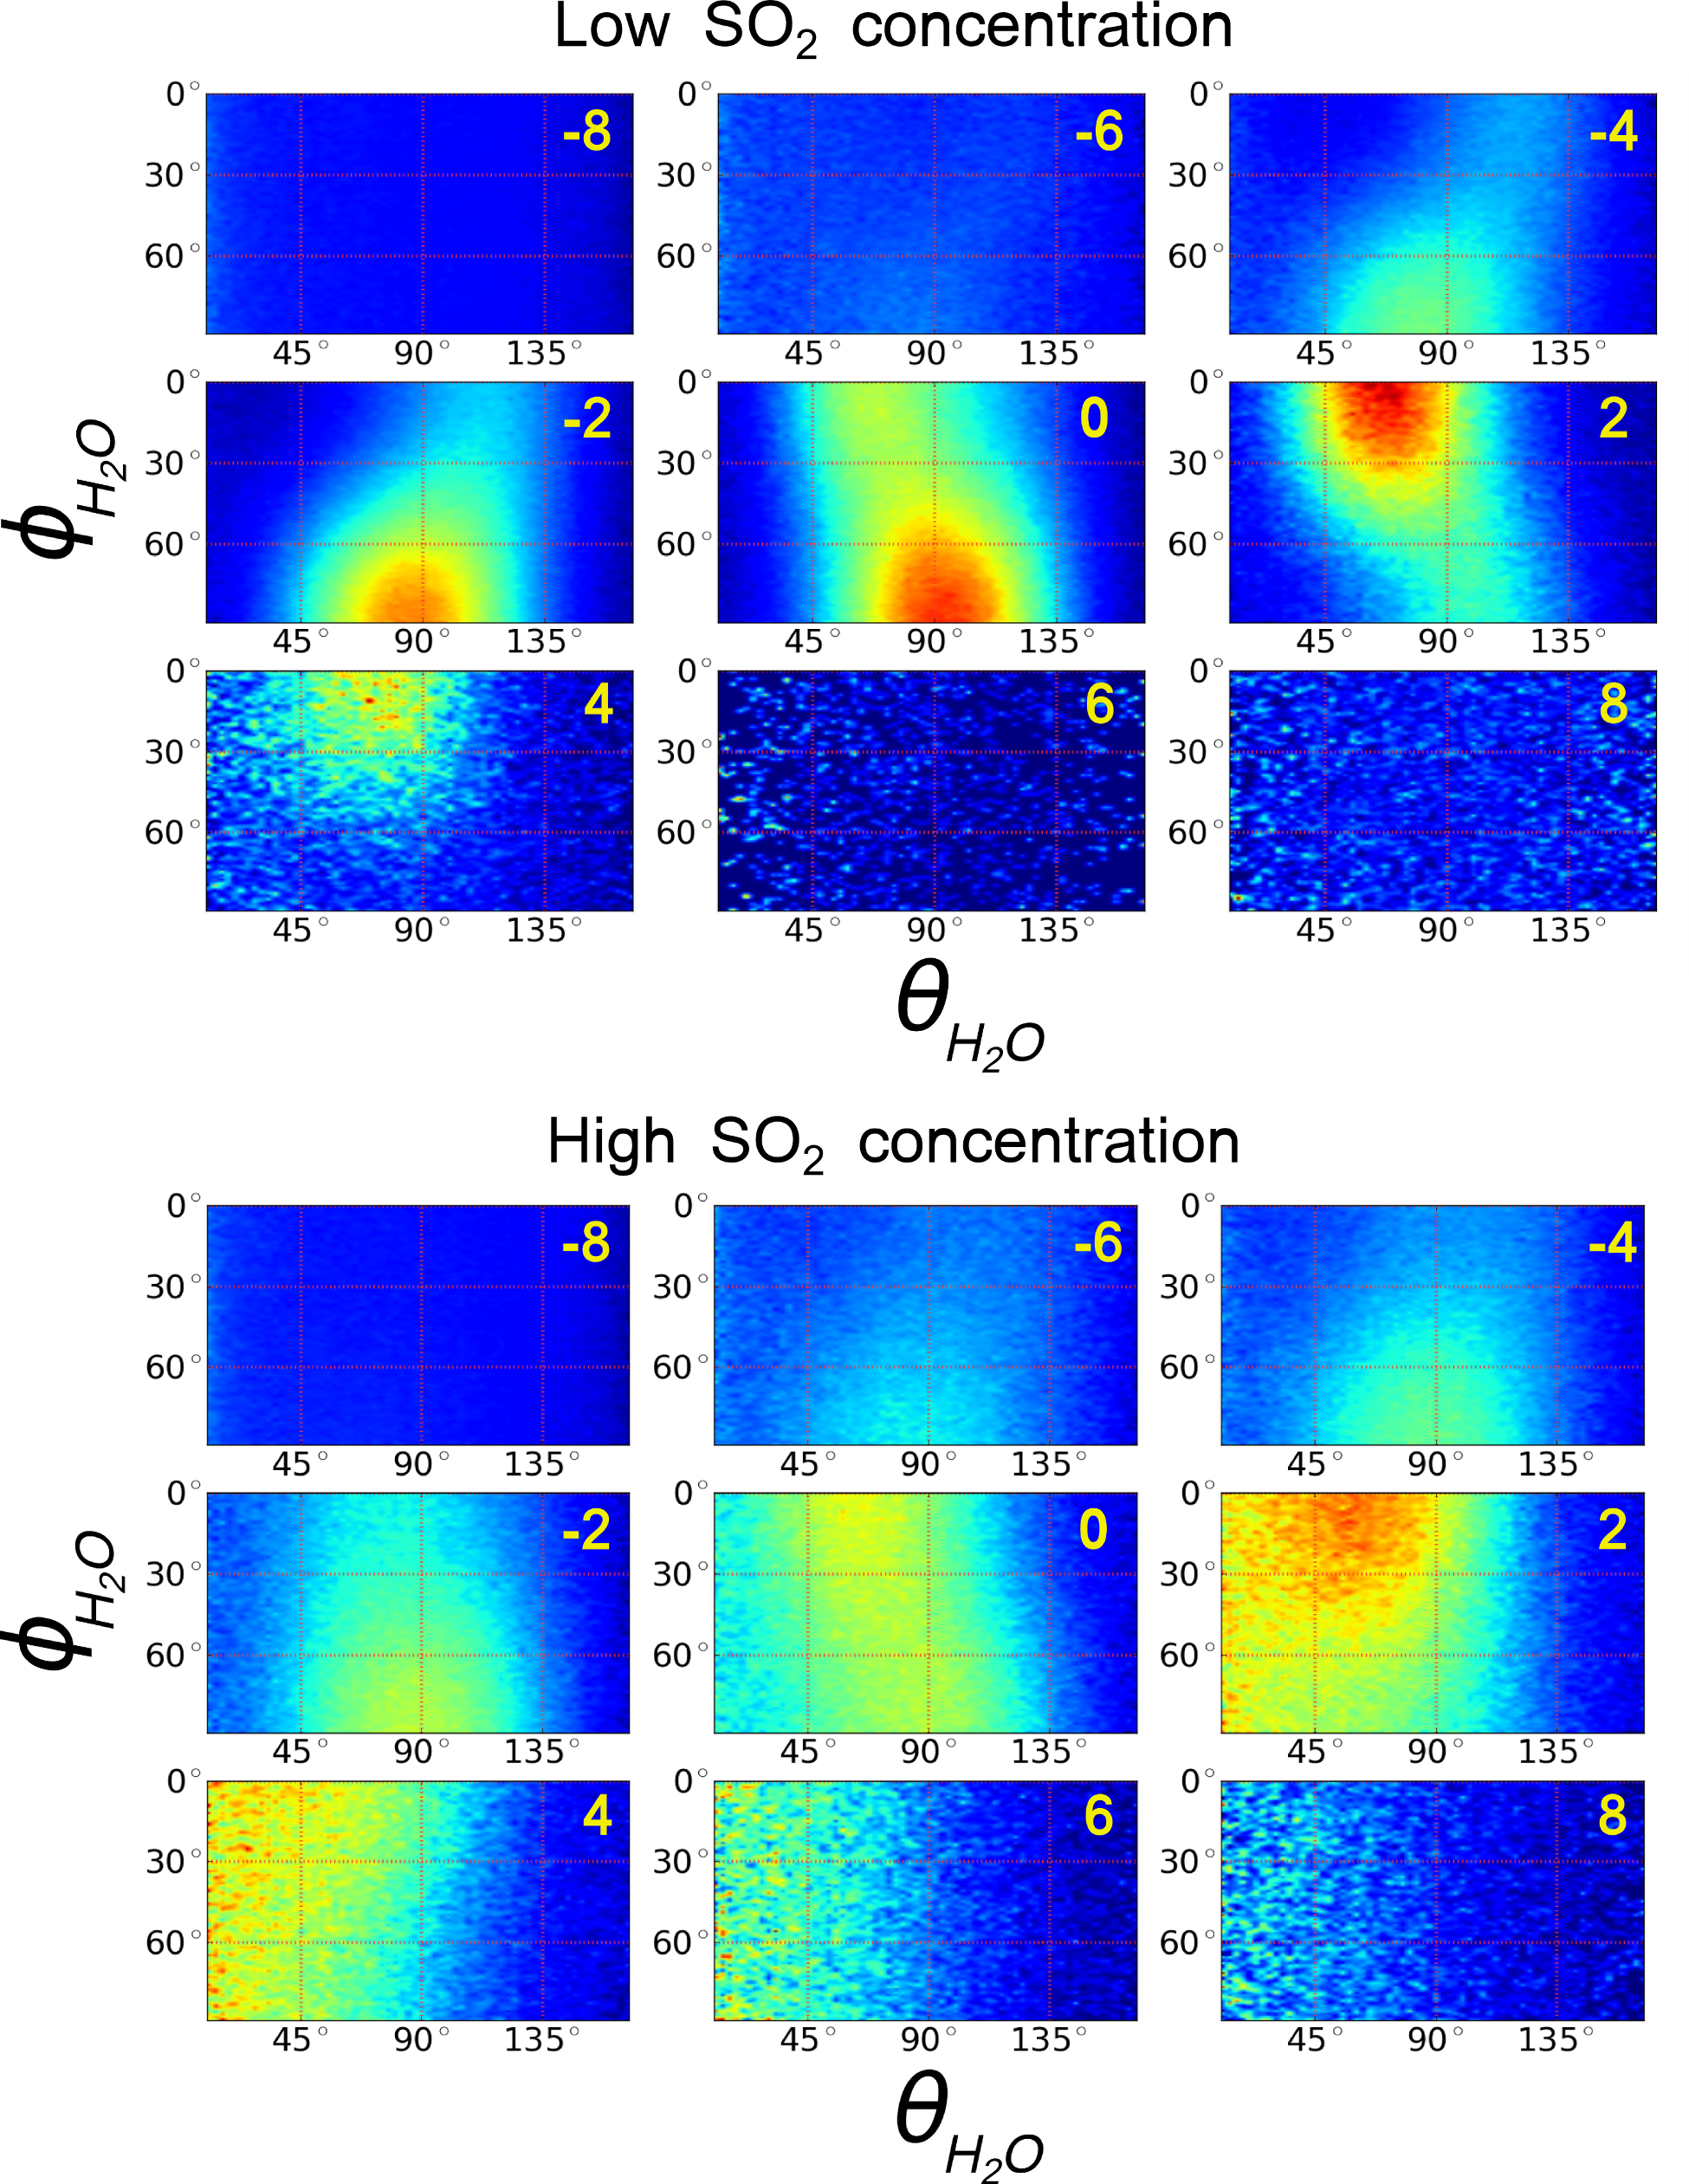
\includegraphics[scale=1.0]{theta-phi-h2o.png}
		\caption{Molecular orientation histograms of \wat~throughout the surface equilibrated systems. The depth (in \angs) of each histogram within the water interface is numbered in the upper-right of each respective plot. The water surface location is set at a position of 0\angs~with negative distance values located in the bulk of the slab, and positive distances towards the gas phase. Each histogram is a bi-variate angle distributions for $\theta$ (horizontal axes) and $\phi$ (vertical axes) in both the neat-\wat~system (top) and the saturated system (bottom). Regions of high intensity are dark red, and low intensity are dark blue.}
		\label{fig:water-orientation}
	\end{center}
\end{figure}


\subsubsection{\suldiox~Orientation}

Orientation distributions of the adsorbed \suldiox~molecules were created during the equilibrium simulations for both the neat-water and saturated systems. Figure \ref{fig:so2-orientation} shows the 2D distributions of $\theta$ and $\phi$ (arranged similarly to the water orientation distributions plots in Figure \ref{fig:water-orientation}). The \suldiox~orientation data set for the neat-water system is much smaller as only a single \suldiox~molecule was simulated in the bulk. The resulting distribution plots are thus representative of the single surface active \suldiox~molecule. The neat-water \suldiox~molecule remains within a narrower region of the interface than the saturated system \suldiox, but effective comparisons can still be drawn. Note that the depth range of the plots in Figure \ref{fig:so2-orientation} is different for the neat-water and saturated systems reflecting the surface mobility of the \suldiox~molecules in the two systems.

In the interfacial region the angular distribution of the single \suldiox~(in the neat-water system) is concentrated primarily in $\theta <$ 90 \textdegree. The peak of the distribution occurs at $\theta=$ 0\textdegree. This indicates that the \suldiox~bisector points out of the water surface, with the sulfur atom pointing towards the aqueous bulk, and the two oxygens pointing into the gas phase. This same distribution occurs in the saturated system for depths below the surface location, $< 0$\angs. Beyond 4\angs~above the surface, both distributions become mostly isotropic, either because the \suldiox~does not venture into the gas in the neat-water system, or because of the nature of the adsorbed \suldiox~layer in the saturated system. Promixity to the water surface highly orients the \suldiox~bisector. % with the sulfur atom pointing in towards the water bulk. %Moving further away from the water surface, and interacting less with \wat~molecules allows for greater orientational freedom as exhibited in the isotropy of the distributions above 4\angs. %Because both the neat-water and saturated systems show rather similar distributions, it is possible that the concentration of \suldiox~does not strongly affect the orientation of the \suldiox, unlike the orientations of waters.

The distributions of $\phi$ are isotropic in both systems at all depths. Because the \suldiox~bisector near the surface is oriented perpendicularly to the interface, the isotropy in $\phi$ is expected. Further from the water surface where the bisector orientation becomes isotropic, the $\phi$ distribution remains isotropic. For the surface \suldiox~orientation, the $\phi$ angle does not provide further information regarding the surface behavior or orientational preference.

%The plots indicate that \suldiox~orients similarly at both the low and high concentration interfacial environments. The $\theta$ values follow similar trends at both concentrations indicating that the \suldiox~sulfur orients down towards the water phase, with both oxygens pointing away from the surface once the \suldiox~is within approximately 5\angs~of the surface. This behavior continues down to at least 5\angs~below the water surface location, notwithstanding any chemical reactions that may occur that are not simulated using the classical MD techniques utilized in this work.

\begin{figure}[h!]
	\begin{center}
		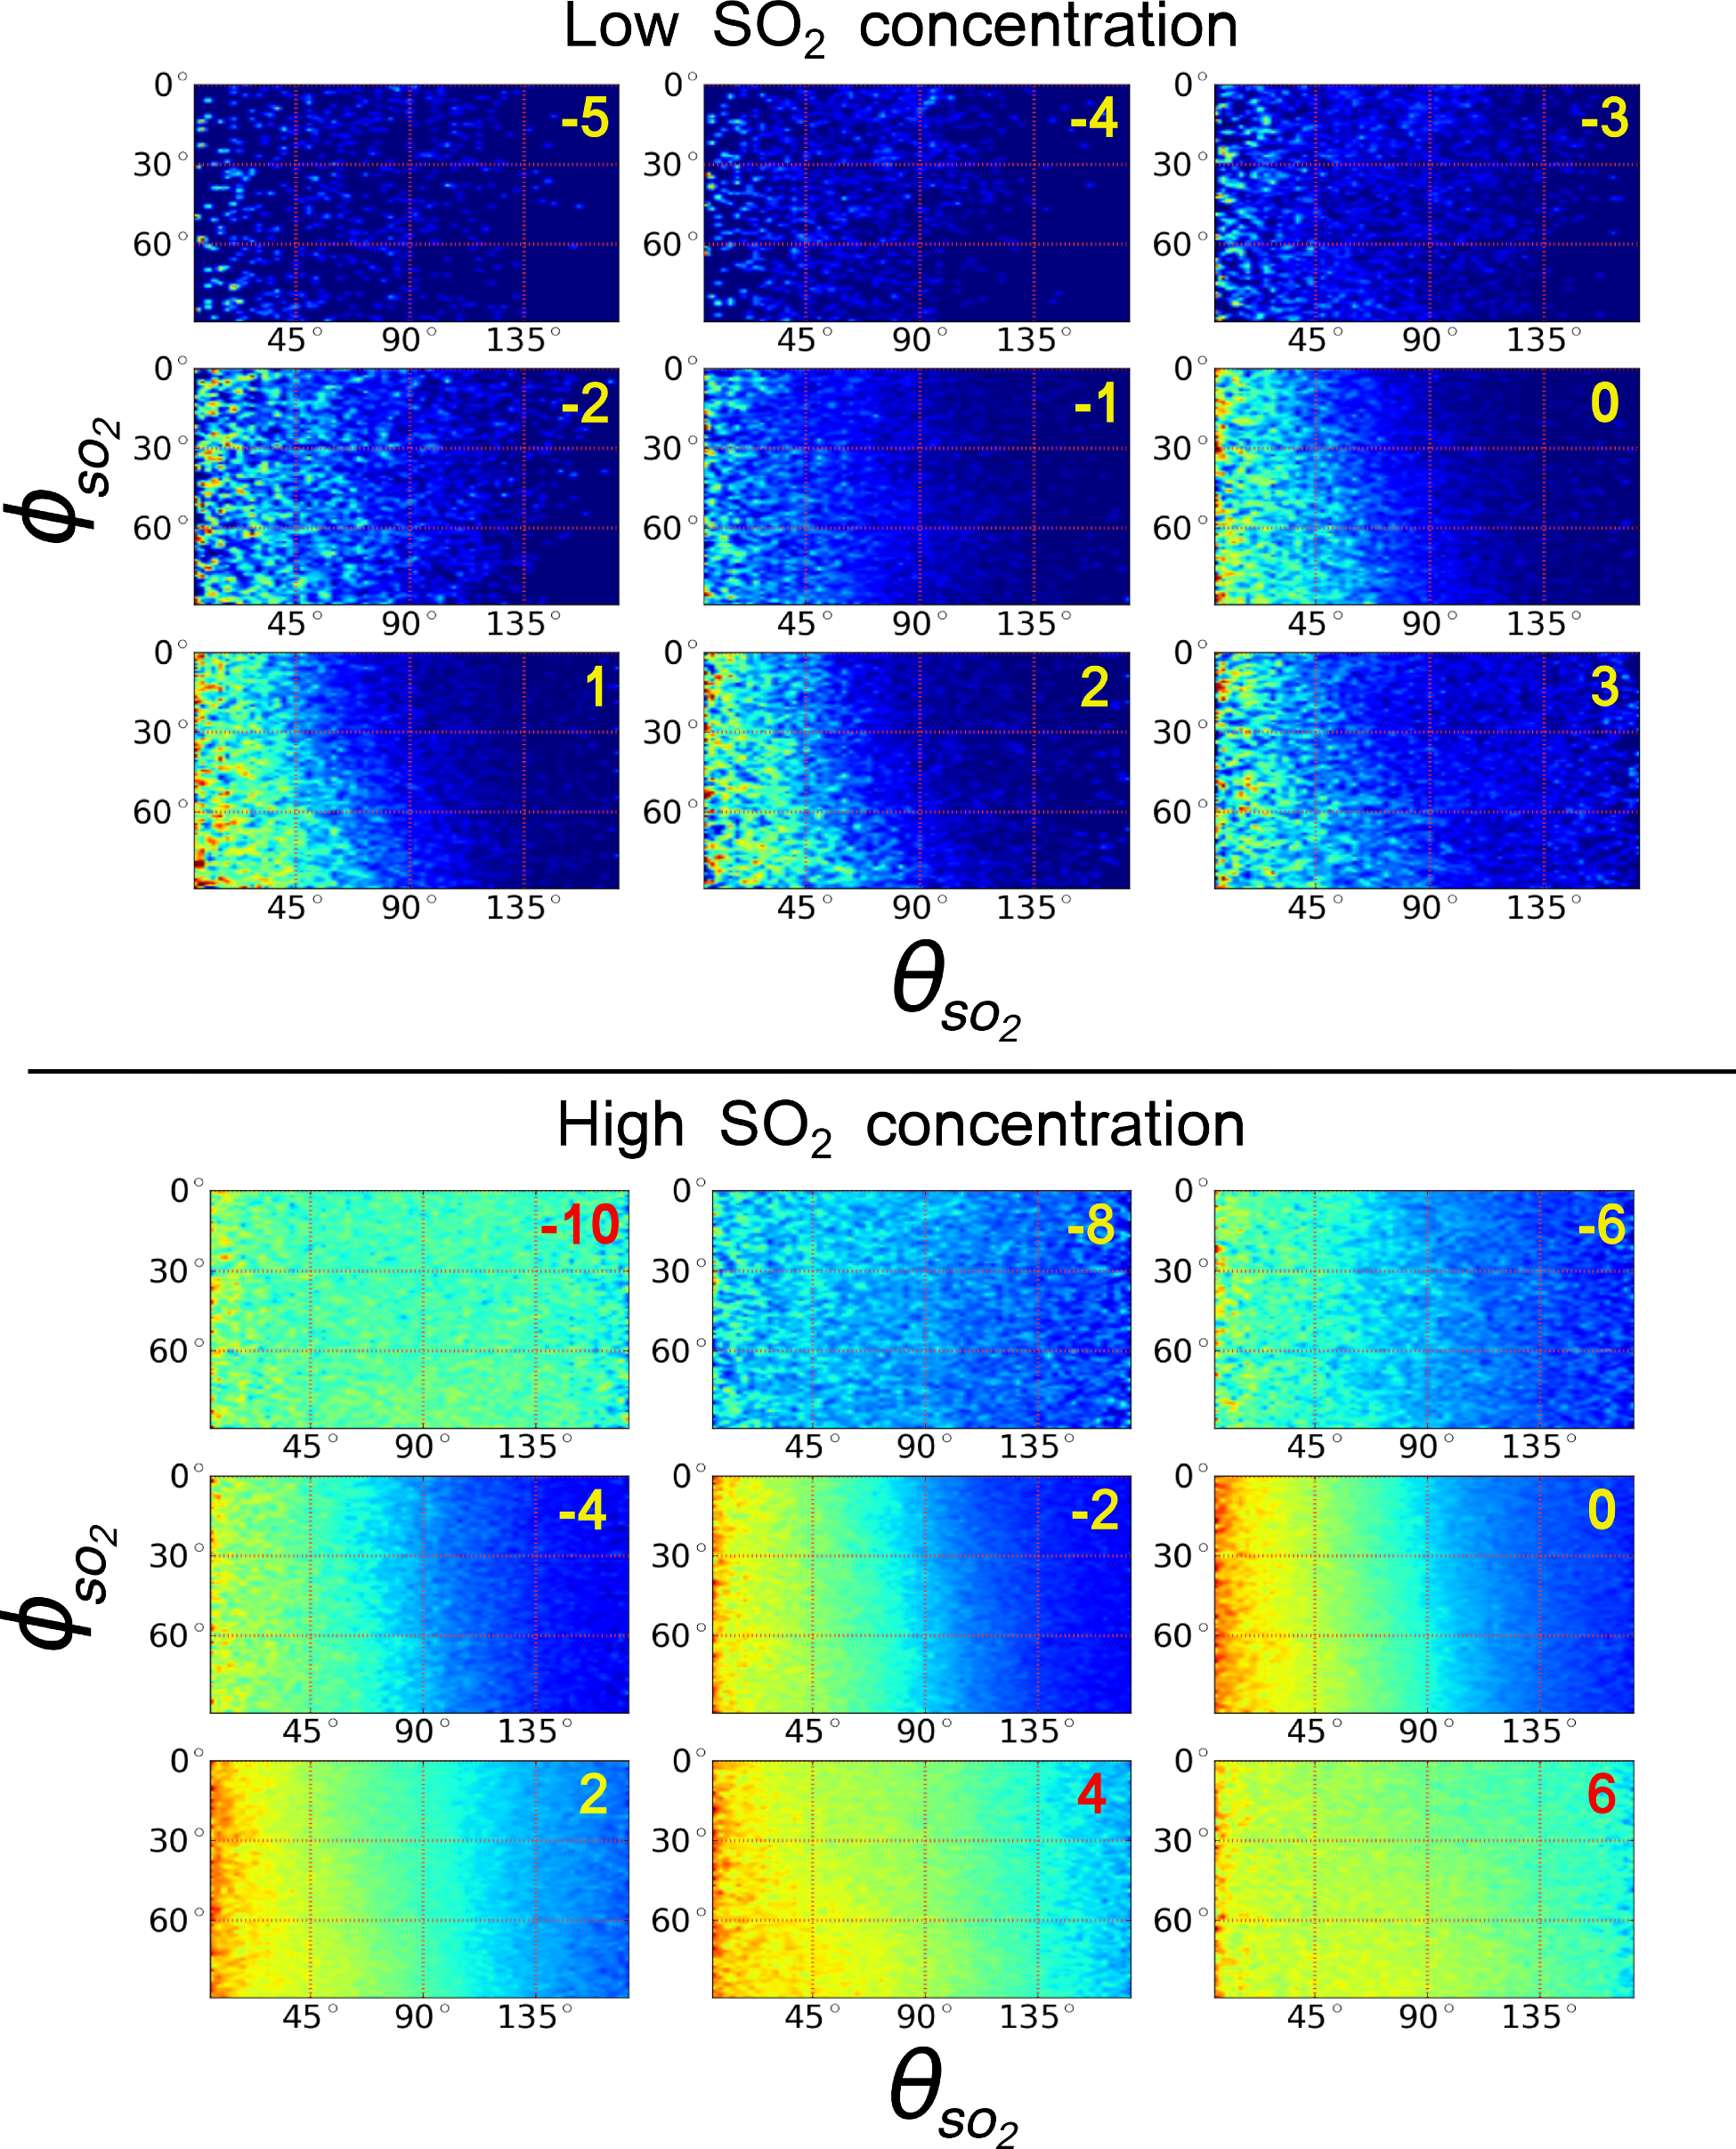
\includegraphics[scale=1.0]{theta-phi-so2.png}
		\caption{Molecular orientation distributions for \suldiox~molecules adsorbed to the water slab surface. The angular distributions are shown for the neat-water (top) and saturated (bottom) systems, and are arranged similarly to the water orientation plots of Figure \ref{fig:water-orientation}. For both systems the distributions show \suldiox~bound to the water surface with the sulfur primarily pointing towards the water slab, and the oxygens pointing to the gas phase. In this configuration the $\phi$ distribution is isotropic because of the water slab's in-plane symmetry. Note that the range of surface depths in the low concentration plot is half that of the saturated system. This is due to the narrower position range of the single \suldiox~molecule.}
		\label{fig:so2-orientation}
	\end{center}
\end{figure}

\subsection{Steered MD Transit Simulations}

\subsubsection {\suldiox~Orientation}

	The orientation of \suldiox~molecules throughout the aqueous adsorption process was monitored during the transit SMD simulations. The angles $\theta$ and $\phi$ of the transiting \suldiox~(Figure \ref{fig:water-angles}) were calculated for each timestep of the SMD simulations as the \suldiox~was pulled into the water slab from the gas phase, both in the neat-water and saturated slab systems. The orientation depth-profiles were collected for the 50 simulations of both systems for various distances from the water surface location, resulting in the 2-dimensional angle and depth-profile histograms shown in Figure \ref{fig:so2-transit-angles}.

\begin{figure}[h!]
	\begin{center}
		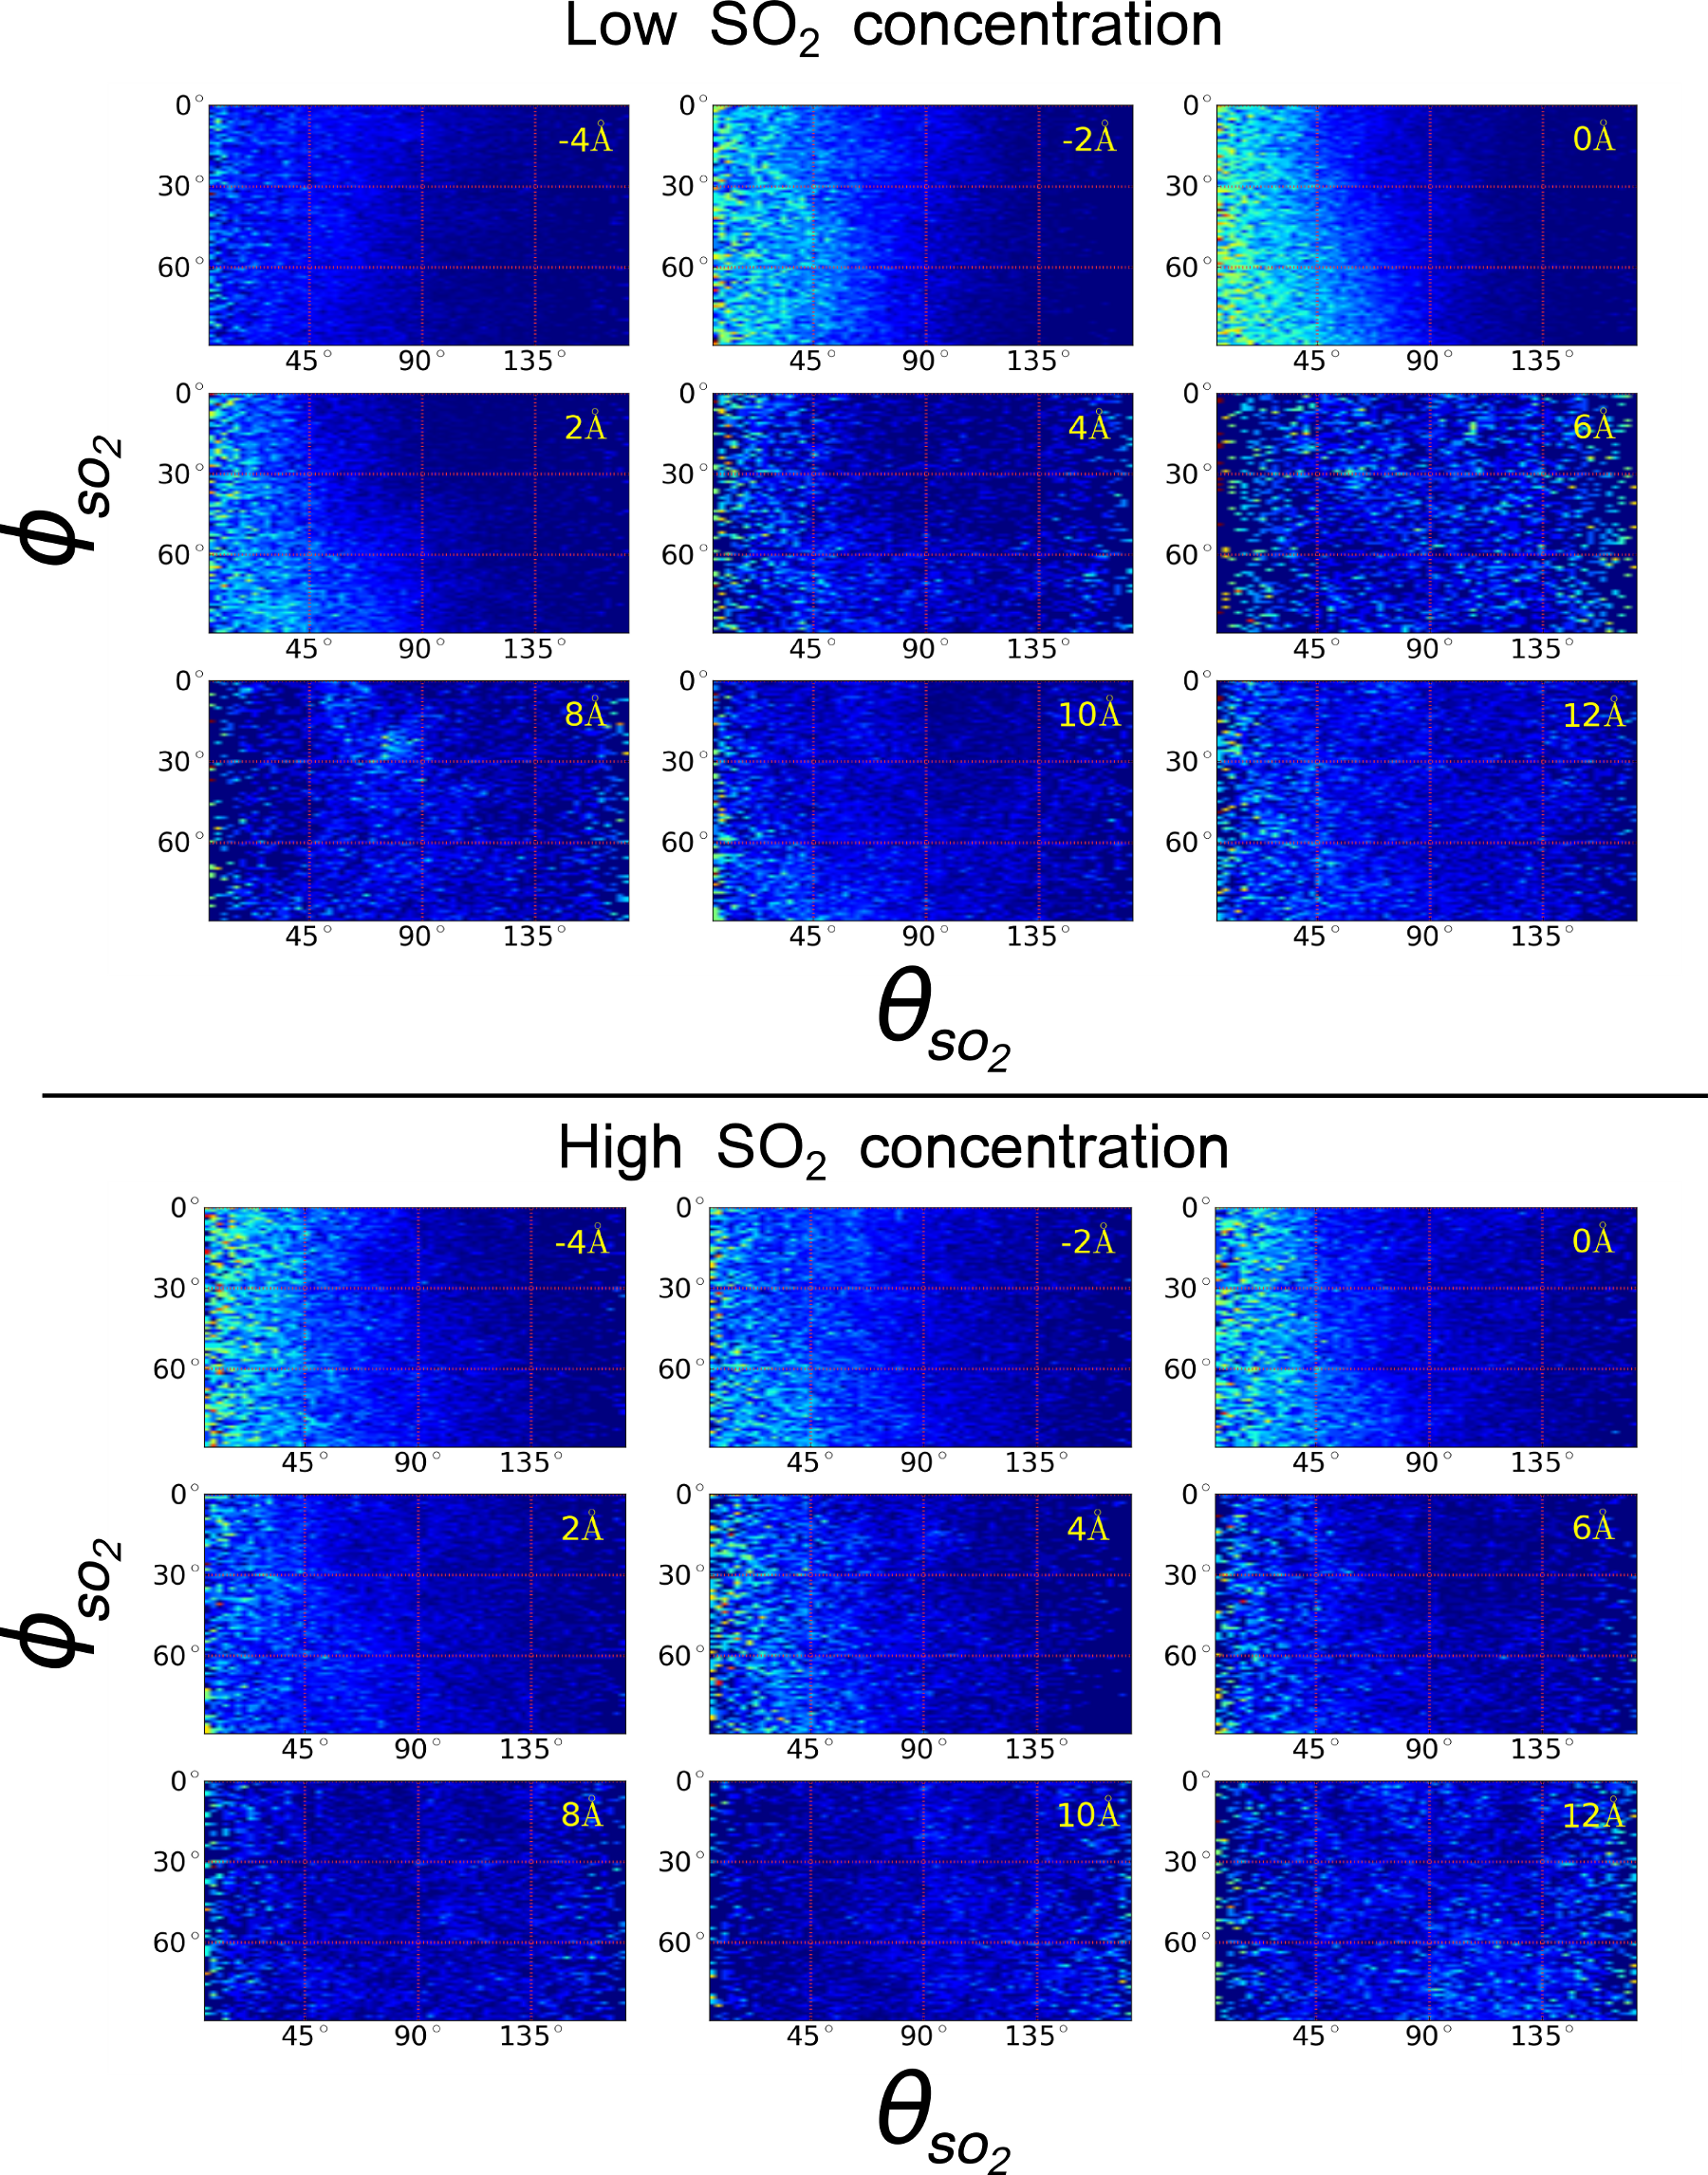
\includegraphics[scale=1.0]{theta-phi-transit.png}
		\caption{Molecular orientation distributions of an \suldiox~at different interfacial depths of an aqueous slab during SMD transit simulations. Both the neat-water (top) and saturated (bottom) data sets were analyzed to determine the angles $\theta$ (horizontal axes) and $\phi$ (vertical axes) of the transiting \suldiox. The distributions shown are those for the single transiting \suldiox~molecule averaged over the 50 SMD simulations.}
		\label{fig:so2-transit-angles}
	\end{center}
\end{figure}

	From its starting position above the water surface, until the \suldiox~moves to within 6\angs~of the water surface location of both systems, the orientation is isotropic in $\theta$ and $\phi$. Isotropic orientation is manifested in the plots as mostly uniform coloration at a given distance from the surface independent of $\theta$ or $\phi$. Near and into the interfacial region the bisector angle $\theta$ becomes more perpendicular to the water surface ($\theta \approx 0$\textdegree) with the \suldiox~sulfur pointing into the water phase, consistent with the equilibrium MD simulation results above. At the point when the \suldiox~reaches the water surface location (0\angs), the bisector is perpendicular to the interface in both the neat-water and saturated systems. %Figure \ref{fig:so2-surface-angles}a depicts \suldiox~near the water surface with the bisector aligned perpendicular to the interface. 
	In the absence of simulated ionic species that form through \suldiox-\wat~chemistry at the surface, it is clear that the adsorbing \suldiox~in the gas phase takes on a preferred orientation to adsorb on a water surface. The main difference between the neat and saturated water systems is where the point of the transition from isotropic to preferred orientations is found. 
 
  % theta differences
  Comparing in more detail the difference in these two systems upon \suldiox~approach, for the neat-water surface, a transition occurs at approximately 4\angs~above the surface water location. Below 4\angs~above the surface, \suldiox~has a preferred net orientation and is close enough to the water surface that it begins to interact with the topmost surface waters. In the saturated system, the same trend occurs, however the onset of the perpendicular orientation begins at approximately 8\angs~above the surface. The layer of adsorbed \suldiox~already present in the saturated system most likely interacts with the transiting \suldiox~molecule. Also, topmost water molecules from the surface move up to a few \angs~inside the adsorbed \suldiox~layer and interact with the transiting \suldiox~further from the surface than those in the neat-water system. It is remarkable that the orientational trend appears so strongly in the $\theta$ plots even with so little data as was collected from the single \suldiox~molecule of each simulation. From onset of orientation above the surface until 10\angs~below (not shown), the \suldiox~holds a preferred orientation.

%\begin{figure}[h!]
	%\begin{center}
		%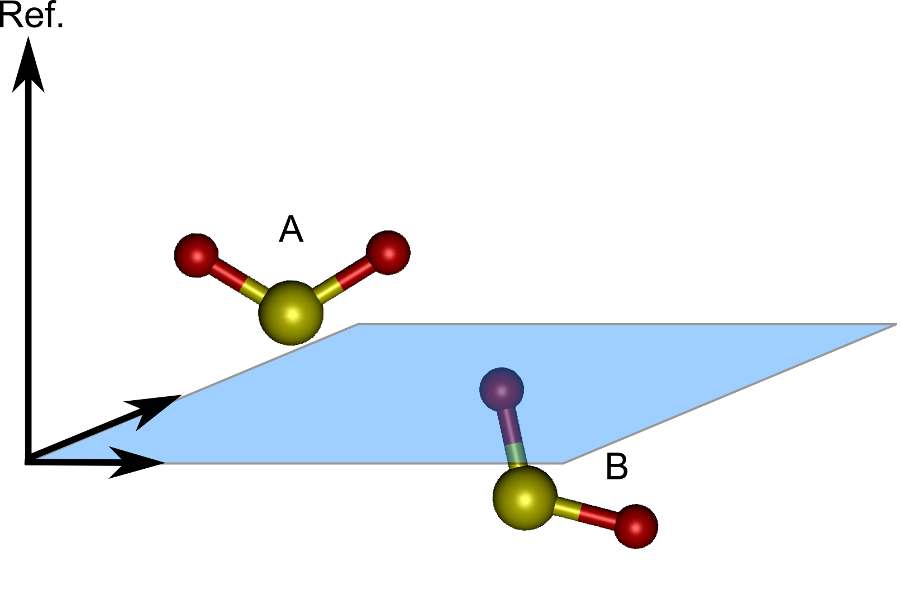
\includegraphics[scale=1.0]{images/angle-cartoons/so2-surface.png}
		%\caption{(A) \suldiox~molecules above and below both neat-water and saturated water surface location orient with the bisectors perpendicular to the interface. The \suldiox~sulfur points down towards the aqueous phase. (B) In the neat-water system, a transiting \suldiox~molecule located below the water surface briefly reorients with one S-O bond more towards the interface above, and the other bond pointing further down into the water bulk.}
		%\label{fig:so2-surface-angles}
	%\end{center}
%\end{figure}

  % phi differences
	%Indeed, the $\phi$ orientations appear mostly isotropic without any clear trends for preferred orientation in that angle. This appears as a mostly uniform color across the entire plot, with minor variations that are disjointed throughout the distance range.

 With a mostly perpendicular bisector angle, it is expected that the values of $\phi$ for \suldiox~would be isotropic relative to the reference axis. This is the case in both systems, with only a few exceptions. In both systems the $\phi$ profiles exhibit mostly isotropic distributions above 0\angs, with several regions of lighter coloration interspersed, but without a clearly formed orientational trend. At the neat-water surface and just above (from 0-2\angs~above the water phase), the $\theta$ profile broadens to $\theta = 90$\textdegree, near $\phi = 90$\textdegree~appearing as a shoulder of light coloration in the bottom-left of the 0-2\angs~axes. This indicates that \suldiox~inclined up to 90\textdegree~from the surface normal will have a preferred $\phi$ orientation lying more flat to the water surface. This is in contrast to \suldiox~molecules above the water surface location, oriented more perpendicularly and without a preference for a particular range of values in $\phi$. The behavior is likely due to the interaction between the waters and the S-O bonds leading to a higher solvation than above the water surface location. As the \suldiox~is solvated by more highly-coordinated bulk water, the S-O bonds experience less equal interaction environments. Baer et al. noted that their force field model for the \suldiox~does not reproduce well the first hydration shell geometries,\cite{Baer2010} so conclusions regarding the specific interactions and hydrate geometries between the \suldiox~and \wat~cannot be made here. It is notable that the same reorientation does not occur as strongly in the saturated system. The presence of the adsorbed \suldiox~layer apparently decreases the reorienting behavior likely because of the disrupting effect the higher \suldiox~concentration has on the water interactions in the interfacial region. %Below this 5\angs~region under the surface, the \suldiox~resumes an isotropic orientation as it becomes fully solvated by bulk waters.

  %Upon approaching the saturated surface at approx. 5\angs, the \suldiox~$\phi$ orientation distribution begins to cluster near $\cos(\phi)=1$, with the $\theta$ distribution remaining more isotropic, but with a trend of $\cos(\theta)>0$. At 5\angs the \suldiox~begins interacting with the other \suldiox~molecules that sit atop the water, and the resulting orientation distribution suggests that contact with the \suldiox~layer causes the adsorbing molecule to lie more flat to the surface. Within this same region from 0-5\angs above the surface, the $\phi$ distribution of the neat-\wat~system remains isotropic. The intensity of the distribution (darker blue) also indicates that the \suldiox~spends little time in this region, as it is quickly adsorbed further into the water bulk.

	%Just below the water surface as the distance moves into negative values, both systems show clear orientational preferences. In both systems the bisector orientation clusters such that $\cos(\theta)<0.5$, with most of the distribution intensity around $\cos(\theta)=1$. This suggests that \suldiox~in a water surface orients with the sulfur pointing into the water bulk, and the oxygens pointing towards the surface water molecules.

	%Differences ocurr between the system orientation profiles once the \suldiox~has moved further than 10\angs below the surface. While both $\theta$ and $\phi$ hold the same trend from just under the surface through to the bulk of the slab in the saturated system, the orientation profile becomes much more isotropic past 10\angs under the surface of the neat-\wat~system. The orientation effect is shallower under the neat-\wat~surface. However, the orientation distribution peaks most intensely, and more tightly clustered with the \suldiox~bisector aligning with the surface normal, just underneath the neat-\wat~surface than the saturated one. The distributions thus show an orienting force extending deeper into the surface of the saturated system than the neat-\wat~system. In terms of how deeply the \suldiox~molecule is oriented, the interfacial region of the saturated system is larger and extends further into the aqueous bulk.

\section {Conclusions}

Gaseous adsorption on solid surfaces has been extensively studied over the past few decades with much learned about how molecular geometry and orientation of the adsorbate are influenced by the proximity of the solid slab.  For a liquid surface where the surface slab is no longer rigid but has molecules with considerable freedom of movement, the surface and approaching gas molecules can be active partners in attaining the optimal geometry and orientation necessary for adsorption and subsequent uptake.    And unlike the solid surface defined by a sharp plane, the interfacial region for the liquid-gas system is much broader, extends on either side of a defined center plane, and is host to a broad distribution of gas-liquid molecular geometries and orientations that change as the gas molecules transit through the interfacial region into the bulk liquid.  Although  our current molecular level understanding of  the complex dances that these molecules play in this fluid interfacial region is in its infancy, emerging studies such as these are beginning to provide unique new insights that are key to understanding many  environmentally important processes at aqueous surfaces.

Presented herein are the results of several classical molecular dynamic simulations that focus on understanding how surface water molecules and adsorbing \suldiox~gas molecules twist and turn as the gas adsorbs and transits the interfacial region. The computational studies emulate and expand on the experimental spectroscopic studies from this laboratory which have found \suldiox~surface complexation at a water surface.\cite{Tarbuck2005,Tarbuck2006,Ota2011}  These spectroscopic studies show clear evidence of \suldiox-water surface complexation but details about this surface complex could only be inferred from spectral changes in the surface water spectrum since \suldiox~could not be monitored directly.   These simulations do not have that limitation and hence can provide information about the behavior of both surface partners and in particular, how their proximity influences the orientation behavior of each other.  The orientational information obtained in these simulations are provided via calculated depth profiles which show the molecular distribution of orientations of the two different interfacial molecules throughout the dimensions of the interfacial region.

Our simulations show that gaseous \suldiox~quickly adsorbs to the water surface and continues to bind until a complete surface coverage is reached. Surface waters reorient in the presence of adsorbed \suldiox. The waters at and just below the interface of a neat-water surface tend to lay flatter to the surface than when a saturating layer of \suldiox~is present. The waters above the surface location or interacting with the layer of adsorbed \suldiox~orient more perpendicularly to the interface, and further expose their ``free-OH'' uncoupled bonds for interactions with \suldiox, and hydrate complex formation. Furthermore, we have found that surface waters underneath a blanket layer of adsorbed \suldiox~will penetrate further into the gas phase, allowing for greater mobility of waters away from the aqueous bulk in the presence of \suldiox.

Through these simulations we also characterize the orientational behavior of \suldiox~during and after adsorption. Our equilibrium neat-water simulations show that a single \suldiox~molecule, representing a low concentration, has a high surface affinity. At a high \suldiox~concentration in the saturated systems, \suldiox~molecules are also surface active, and are found further out of the water phase than at the lower concentration. These \suldiox~molecules form a bound layer that crowds the surface and interacts with the surface waters. The orientation of \suldiox~on the water surface was found to be similar for both low and high concentrations. Those \suldiox~molecules at or below the surface water location strongly orient with the sulfur atom pointed in towards the water bulk, and the oxygen atoms out towards the gas phase. The \suldiox~molecules slightly above the water surface lose this net orientation within 6-8 \angs. Those  molecules further from the water are more isotropically oriented. Figure \ref{fig:so2-surface-cartoon} depicts what the neat-water and saturated surface molecules look like for both \suldiox~and \wat~orientations and locations based on the calculations.


\begin{figure}[h!]
	\begin{center}
		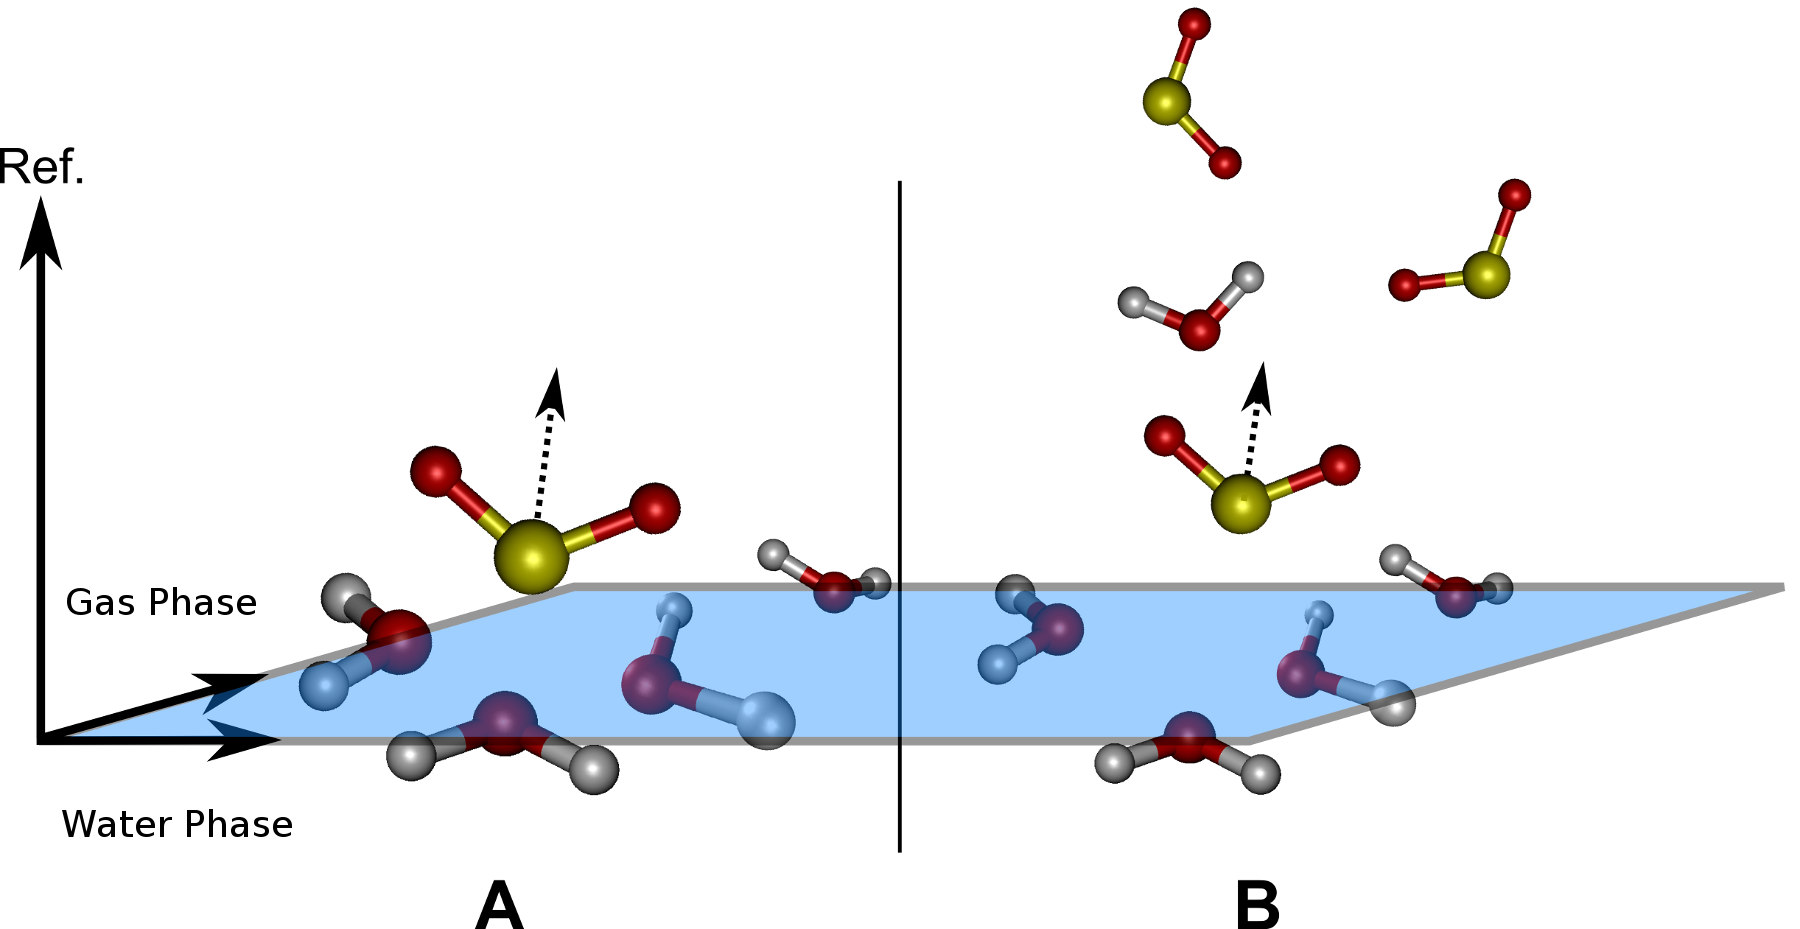
\includegraphics[scale=1.0]{system-surface.png}
		\caption{\wat~and \suldiox~both exhibit preferred orientations in the region near the liquid-gas interface. The neat-water system (A) with a single \suldiox~molecule (low-concentration) has surface waters orienting mostly flat to the interface. When the \suldiox~concentration is increased, as in the saturated system (B), the waters at the surface behave similar to the neat-water interface, but waters that venture into the adsorbed \suldiox~gas layer orient strongly with their bisectors pointing out from the aqueous phase towards the gas. In both cases, the \suldiox~orients with its molecular bisector pointing out to the gas phase when it is near the surface, and isotropically further into the gas phase. Sulfur, oxygen and hydrogen atoms are colored yellow, red, and white, respectively.}
		\label{fig:so2-surface-cartoon}
	\end{center}
\end{figure}

Steered molecular dynamics simulations were used to model the behavior of an adsorbing \suldiox~as it moves from the gas phase above the water down through the surface and into the bulk. The \suldiox~reorients as it makes its first contact with the water interface. Within 4 \angs~of the surface the \suldiox~is mostly oriented with its sulfur towards the water phase. The results for the transit through the interface show that in both systems of low and high \suldiox~concentration an adsorbing \suldiox~near the interface has very similar orientation to those molecules already bound to the water surface. The \suldiox~pulled further into the water bulk retains its orientation until it is past the interfacial region and then isotropically orients with the bulk water.

These studies provide a starting point for future studies in this area that seek to understand how gases of different concentrations and chemical composition adsorb and transit across an aqueous/air interface. Obtaining such knowledge will be invaluable for understanding many environmental aerosol and land water systems where gaseous uptake at a water surface does not conform to expectations.\cite{Jayne1990,Yang2002,Worsnop1989,Boniface2000} Investigations of these and related low-temperature effects will be forthcoming in future publications.

% In such cases, surface complexes are often invoked with little direct evidence of the formation of such complexes. 

%Having now examined the transition of \suldiox~from the gas to adsorbed aqueous phases, we are better able to research the many questions remaining of adsorption and interfacial chemistry of gas molecules. What species form during the adsorption transition, and how do molecular properties affect the process? Can we form a theory that will more fully explain the transit of many small molecules of environmental and industrial interest? This study is one of several characterizing \suldiox~adsorption and behavior on aqueous surfaces. We plan to report further results of ongoing computational simulation and experimental studies regarding temperature and chemical constituent effects on atmospherically relevant water surfaces.

\bibliography{bib/SulfurDioxideText}

\end{document}
